\section{Logistic regression with latent spatial variables}

This section considers augmenting logistic regression models with a spatial field of random variables. The latent variables are represented by a multivariate Normal distribution with an element corresponding to each pixel. The correlations of the latent variables allow correlations between nearby probabilities of rainfall.

\begin{figure}[t!]
\centering
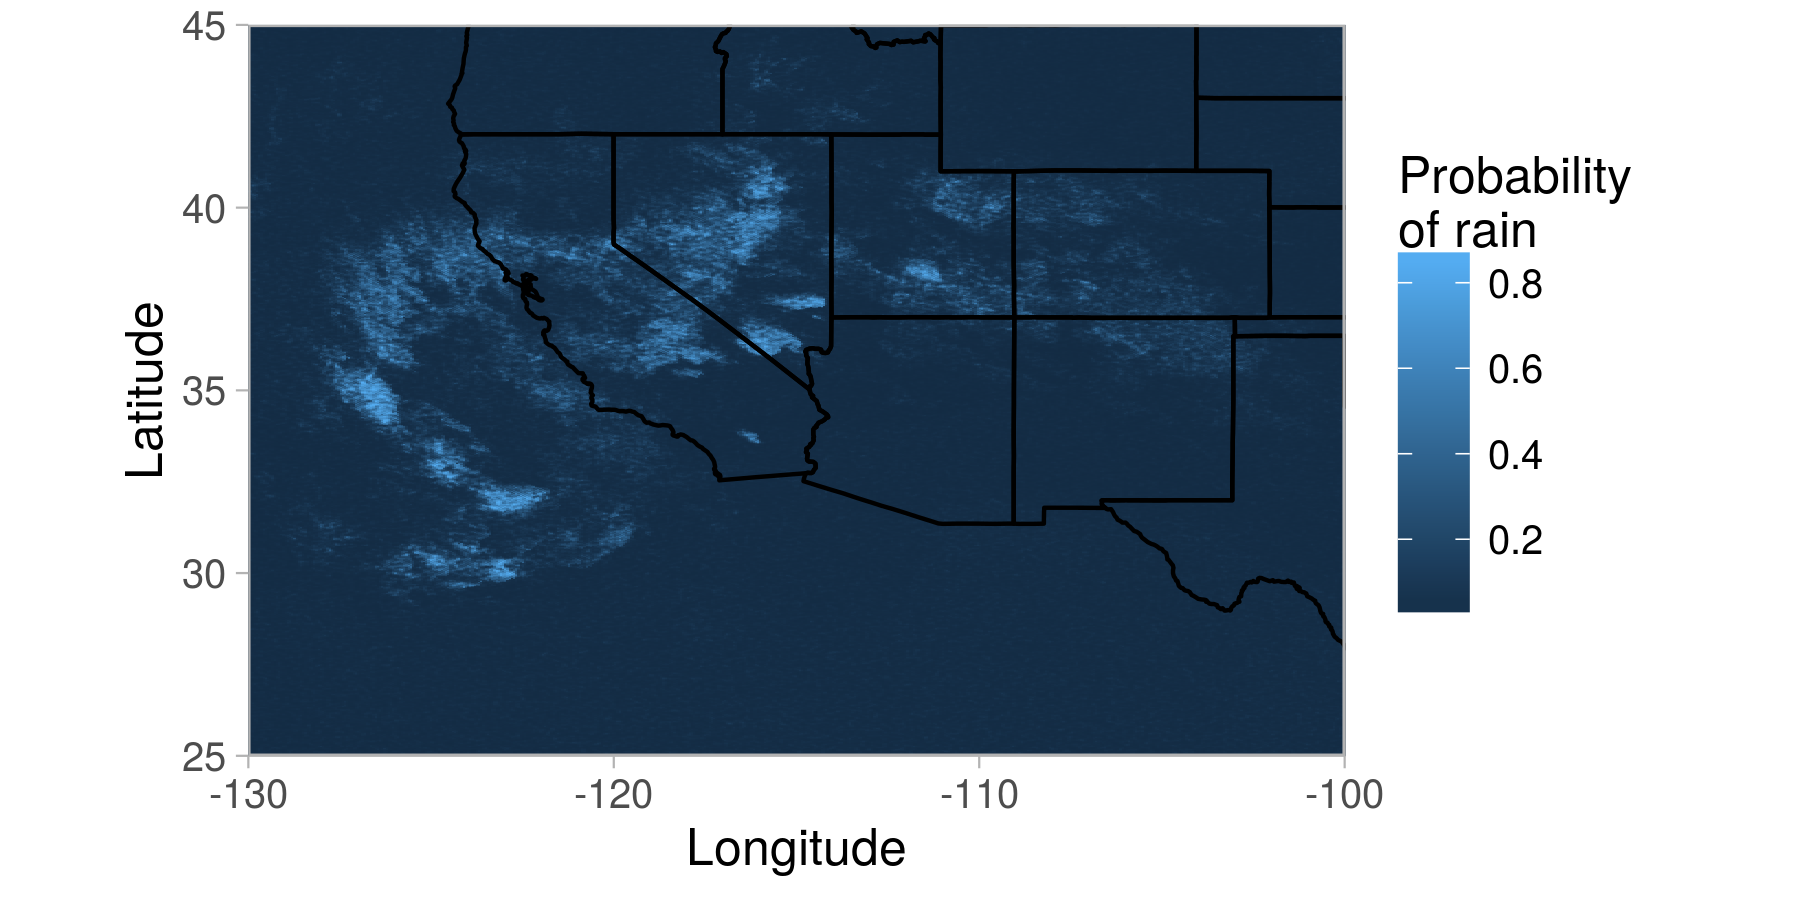
\includegraphics[height=2.8in]{./R/prec.png}
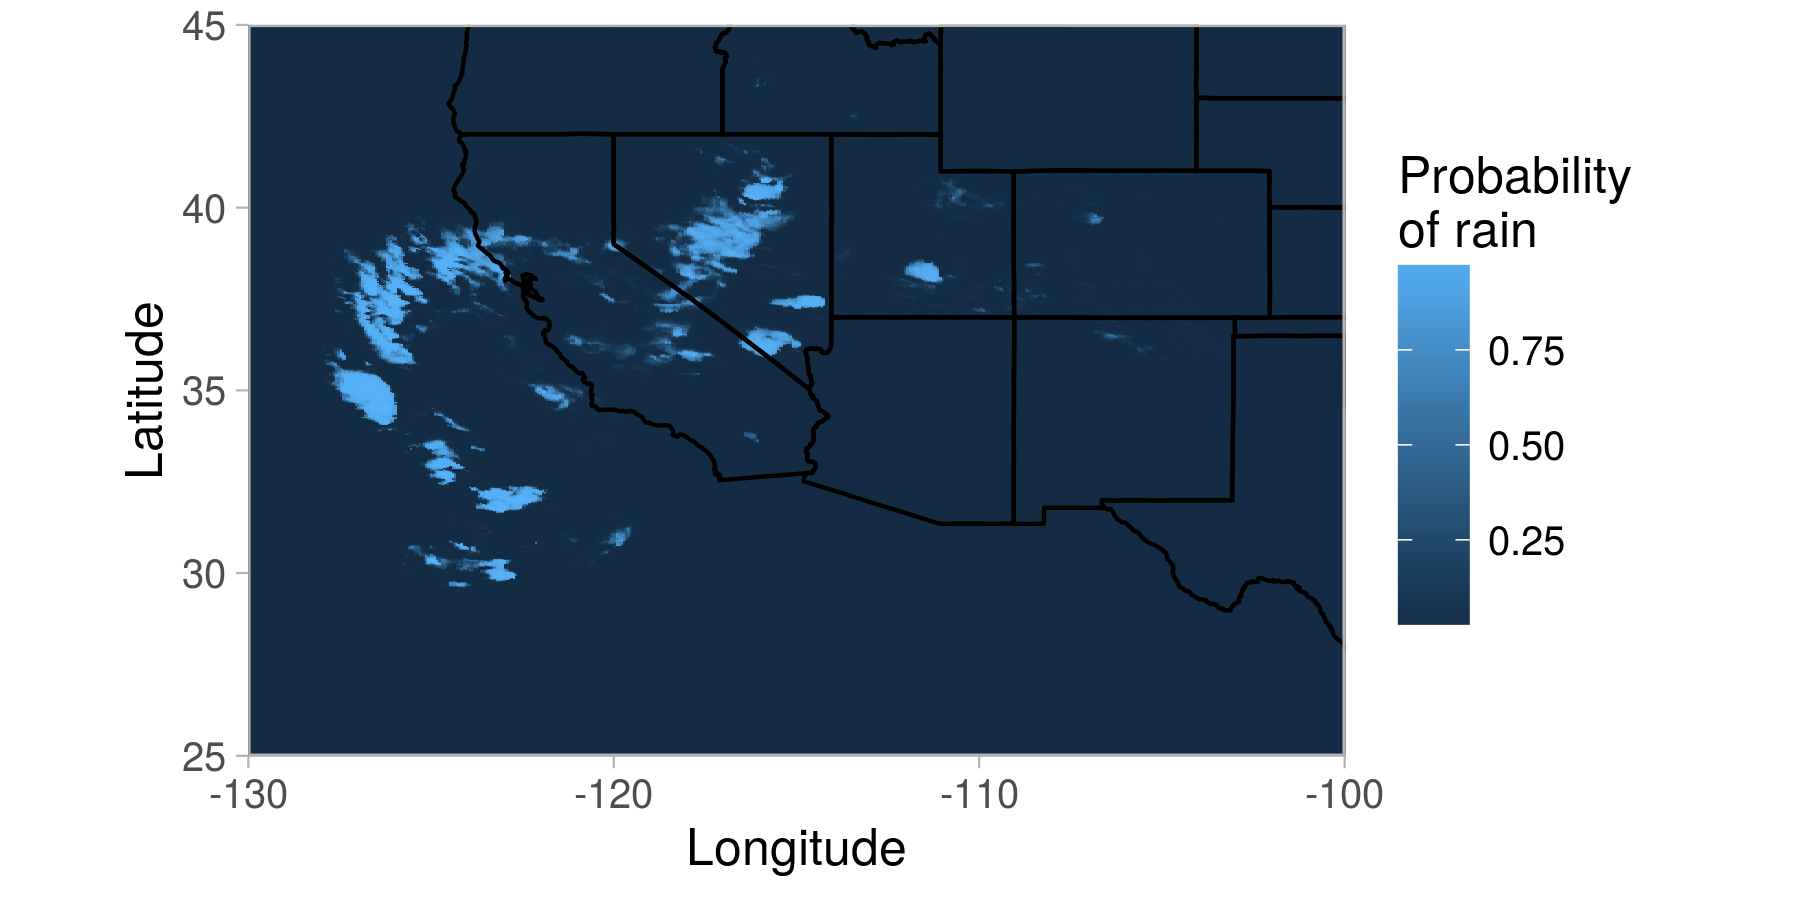
\includegraphics[height=2.8in]{./R/prec_w.png}
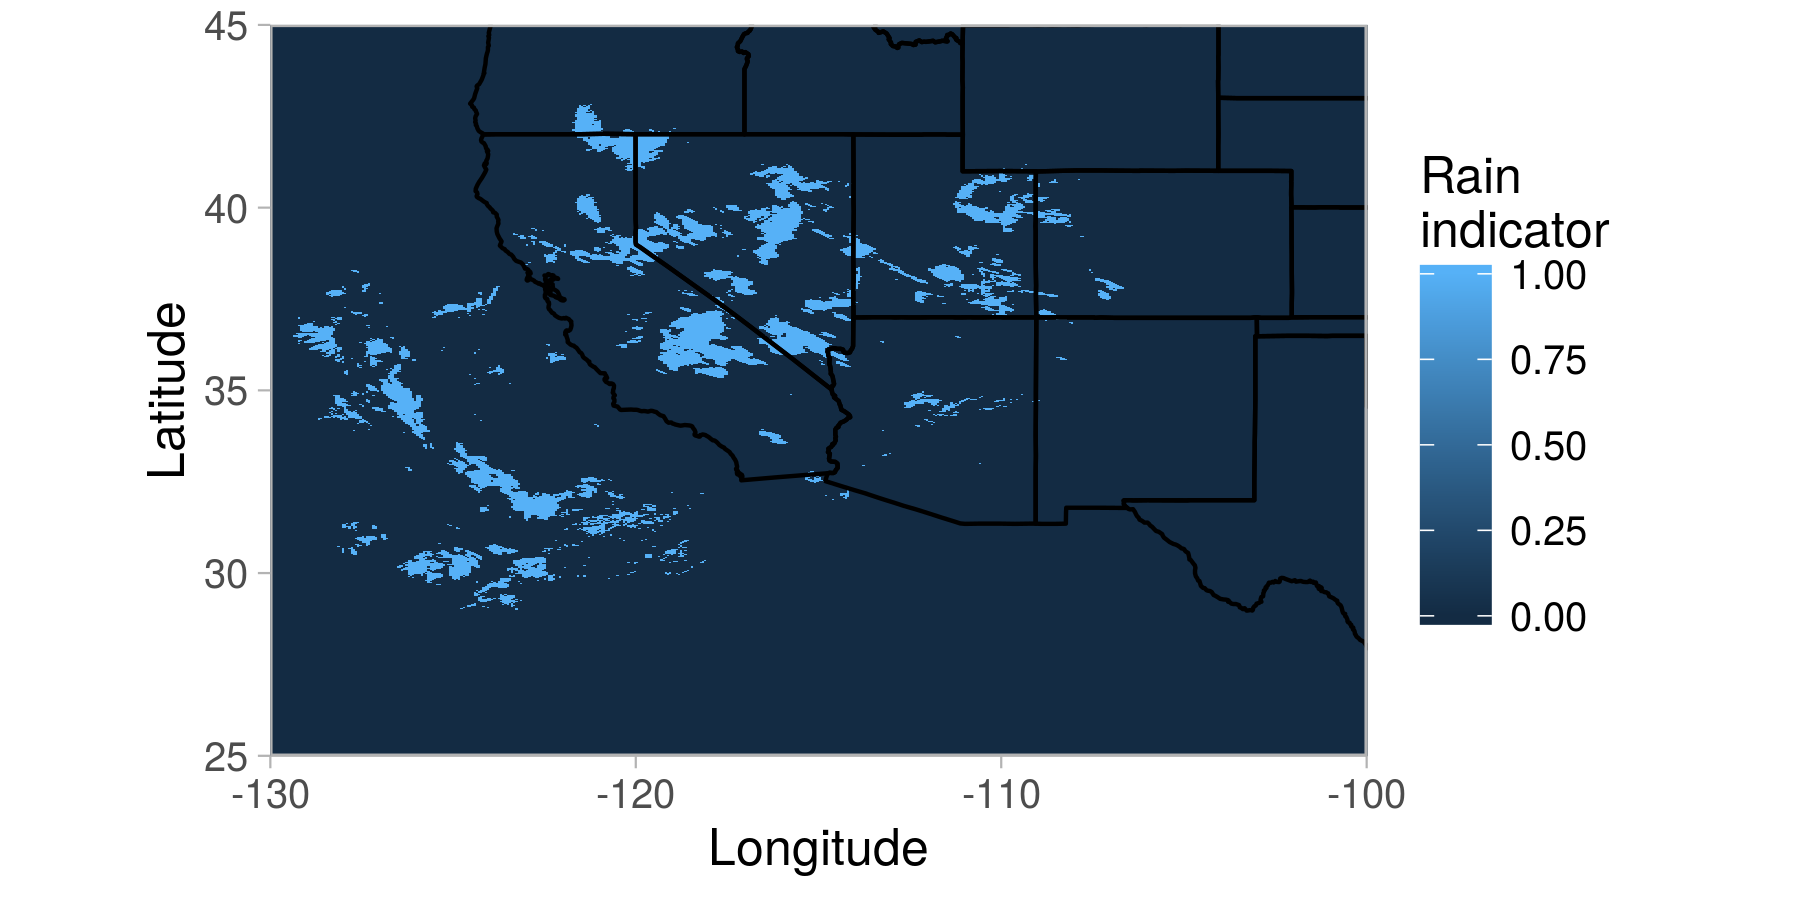
\includegraphics[height=2.8in]{./R/prec_t.png}
\caption{Maps of rainfall probability given by the two latent variable LR models. Top is LR-CRF and bottom is LR-CRF+. Rainfall is of September 12, at 5:45am.}

\label{probprec}
\end{figure}

\subsection{Description}

\subsubsection{Logistic regression (LR)}

Let the probability of rainfall at cell be $p_i$, $i=1,\ldots,n$, and the occurrence of rainfall be $Z_i$ distributed $Bernoulli(p_i)$. In this model we only consider a single explanatory variable, the temperature at each pixel, $T_i$. The standard logistic regression (RL) on $p_i$ is

$$
logit(p_i) = \beta_0 + \beta_t  T_i
$$

where $logit(x)=log(x/(1-x))$. Rainfall has strong spatial correlation, which can be introduced to the LR model by incorporating a Gaussian conditional random field (CRF). 

\subsubsection{Simple Gaussian Markov Random Field (LR-CRF)}

The CRF component, $W$ describes the strength of the spatial correlation of rainfall. Let $W$ have a multivariate Gaussian distribution with $n$ components, $Normal(0, \Sigma^{-1})$. The covariance matrix $\Sigma$ is parameterized by a sparse precision matrix $\Sigma^{-1}$ in which the the entries are nonzero only if two pixels are adjacent in the image. The model can now be written

$$
logit(p_i) = \beta_0 + \beta_t T_i + w_i.
$$

In geostatistics this is called a Conditional Autoregressive (CAR) model \cite{Waller2010}, and the $W$ is interpreted as a type of random effect on the intercept. Then the joint distribution on the CRF $W$ is equivalent to defining the conditional distributions \cite{Besag74}. Specifically,

$$
w_i | w_{j \neq i} \distas{} \, Normal\left( \frac{1}{m_i} \sum_{j \in n(i)} w_j, \frac{\tau^2}{m_i} \right),
$$

where $n(i)$ is the set of neighbors of pixel $i$, and $m_i=|n(i)|$. For the grid adjacency matrix the size of the nieghborhood is $m_i=4$ for interior pixels and $m_i$=2 and 3, respectively, for corner and edge pixels. When the precision matrix is sparse, which is the case for the rainfall data, sparse matrix operations on the precision matrix can drastically reduce the computational burden of inference in CAR models. In the case of this data it would not have been possible to naively store the precision matrix in memory.

\subsubsection{Repeated LR with Gaussian Markov Random Field (LR-CRF+)}
A two-stage latent variable model was motivated by the physical necessity of clouds for rain to occur. Although estimates for clouds were available, we desired a joint probabilistic model for cloud pixels as well as pixels in which rainfall ocurred. Temperature, however is still the only covariate. Clouds can be easily distinguished from ground because they are cooler.

Simply conditioning on a pixel belonging to a cloud might improve the model. Furthermore, the LR parameters for rainfall might well depend on whether or not the pixel belongs to a cloud. This model is relatively ad-hoc, but the intuition is that the latent field is placed on the LR for determining cloudiness, and a further LR predicts rainfall. Roughly, $P(rain, cloud)= P(rain| cloud)*P(cloud)$. The model here specifies rainfall probabilities $p_i$ as

$$
p_i = logistic(\beta_0 + \beta_t T_i + w_i)  logistic(\beta_p + \beta_{pt} T_i),
$$

where $logistic=logit^{-1}=\exp{x}/(1+\exp{x})$. The Gaussian Markov Random Field $W$ is structured in the same as in the LR-CRF model.

\subsection{Implementation}
A Bayesian analysis with weakly informative priors on $\beta$ was performed using the Stan probabilistic programming language. Only \emph{maximum a posteriori} estimates were estimated. The three models described above were compared using several different metrics. Note that these experiments are qualitatively different from the earlier ones because these results are from in-sample predictions. However these are still useful for comparing how well different models describe the in-sample data.

\subsection{Results}

\begin{table}[ht]
\centering
\begin{tabular}{lrrr}
  \hline
Model & Overall rain proportion & Sensitivity & Specificity \\ 
  \hline
LR & 0.006 & 0.068 & 0.997 \\ 
  LR-CRF & 0.008 & 0.171 & 0.999 \\ 
  LR-CRF+ & 0.039 & 0.310 & 0.972 \\ 
   \hline
   Truth & 0.040 & 1.000 & 1.000
\end{tabular}
\end{table}

The two latent variable models were compared to a baseline logistic regression model. Numerical results are found in Table 1. The LR-CRF model made small but nontrivial improvements above the LR model, by all three metrics under consideration. This might indicate that taking into spatial structure has benefits. The LR-CRF+ model is notable for having by the most well-calibrated overall proportion of predicted rain, and also for having the highest sensitivity to rain. However these improvements come at the cost of a small decrease in specificity. Finally, as seen in the example maps of Figure 3, the LR-CRF+ model produces the most realistic-looking maps qualitatively. For example the LR-CRF+ produces sharper edges on its estimates of areas with rainfall.

It is also interesting to compare the parameter estimates between the models. Table 2 summarizes the two common $\beta_\cdot$ parameters between the 3 models, and also the the spatial correlation parameter $\tau$ for the two latent variable models. The LR and LR-CRF have similar estimates while the LR-CRF+ model has estimates with greater magnitude. Since both LR-CRF and LR-CRF+ had Normal priors, essentially penalizing parameters with $l_2$ loss, this might suggest that LR-CRF+ found more evidence in the data for greater parameter values. Although it performed better than LR-CRF in most regards, LR-CRF and LR-CRF+ agree closely on the spatial correlation $\tau$. 

\begin{table}[ht]
\centering
\begin{tabular}{lrrr}
  \hline
Model & $\beta_0$ & $\beta_1$ & $\tau$ \\ 
  \hline
LR & -3.927 & -1.091 & $\cdot$ \\ 
LR-CRF & -3.866 & -1.051 & 0.841 \\ 
LR-CRF+ & -5.235 & -2.126  &  0.861 \\ 
   \hline
   Truth & 0.040 & 1.000 & 1.000
\end{tabular}
\end{table}

\subsection{Conclusion}
This section has explored several latent variable models for rainfall. Model fits for two models based on logistic regression paired with Gaussian Markov random fields. These latent variables models were compared to a baseline logistic regression model. The latent variable models demonstrate potential for improvements over baseline logistic regression, but none of the models considered in this section perform well in an objective sense.

Moreover, in this work they are not useful for predicting out-of-sample. For out-of-sample predictions it may be interesting to consider a spatio-temporal model for the latent variable in which they use Kalman-filter style updates at each time step. Another reflection of the same problem is the limitation that the model results tend to be unstable due to the latent variables. The estimates of latent variables may become much more stable if they are smoothed between past and future time periods.